\section{Solución propuesta}
La solución propuesta consiste en SheetMusic, una plataforma web progresiva (PWA) basada en inteligencia artificial (IA) diseñada para la enseñanza adaptativa de teoría musical. El sistema busca resolver la fragmentación horaria y heterogeneidad del conocimiento en el aula chilena mediante un entorno gamificado. La plataforma articula tres actores clave: la experiencia de aprendizaje del estudiante guiada por un grafo de conocimiento no lineal, las herramientas de seguimiento pedagógico para el docente, y un microservicio adaptativo impulsado por Aprendizaje por Refuerzo Profundo (DRL).

\subsection{Arquitectura distribuida}
El sistema adopta el paradigma de arquitectura de microservicios distribuidos, separando la lógica de presentación, la capa de persistencia/autorización y el cómputo intensivo de Inteligencia Artificial. La Fig.~\ref{fig:arquitectura} ilustra este diagrama de componentes distribuidos que garantiza escalabilidad horizontal y alta disponibilidad.

\begin{itemize}
    \item \textbf{Capa de Cliente (Frontend):} Desarrollada con Ionic React v8 y Capacitor v7. Es una PWA instalable nativamente. Utiliza React Query para la gestión del estado remoto y peticiones HTTPS/RESTful autenticadas (JWT).
    \item \textbf{Capa de Servicios de Backend (BaaS):} Supabase sobre PostgreSQL 15. Administra identidades, historial de progreso, telemetría y aplica políticas RLS (Row Level Security).
    \item \textbf{Capa de Inteligencia (Motor DRL):} Construida con FastAPI, PyTorch y Stable-Baselines3. Procesa el estado del estudiante y devuelve la recomendación de ejercicios.
\end{itemize}

\begin{figure}[htbp]
    \centering
    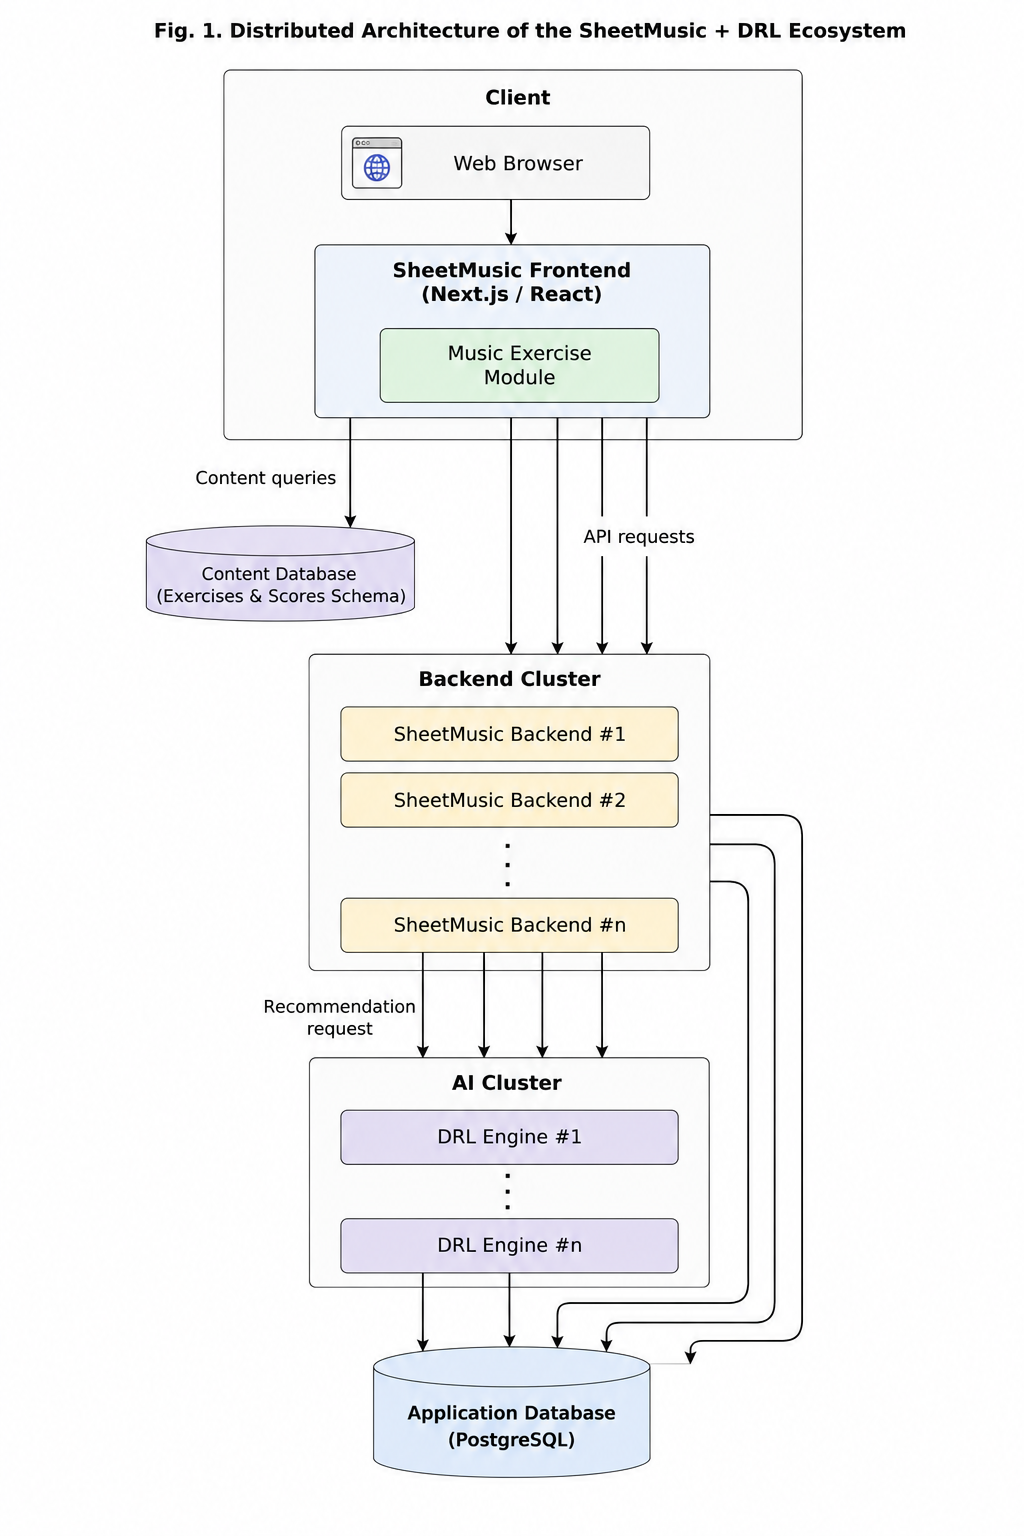
\includegraphics[width=0.49\textwidth]{Imagenes/fig_arch_system.png}
    \caption{Diagrama de arquitectura distribuida del ecosistema SheetMusic + DRL.}
    \label{fig:arquitectura}
\end{figure}
\subsection{Funcionamiento de Módulos e Interacción Distribuida}
La experiencia del estudiante se estructura en dos módulos principales diseñados para desacoplar la lógica de presentación de la persistencia de datos y el cómputo de inteligencia artificial.

\subsubsection{Renderizado Dinámico de Contenidos Pedagógicos}
El objetivo del módulo de material de aprendizaje (Fig.~\ref{fig:material_aprendizaje}) es proveer una lección teórica estructurada según la unidad del grafo seleccionada. Para lograr esto sin acoplar la interfaz gráfica a estructuras rígidas, el cliente invoca procedimientos almacenados remotos (RPC) en el backend de Supabase. La base de datos responde enviando la lección encapsulada en un formato de datos semiestructurado de tipo \texttt{JSONB}. El motor de renderizado del frontend interpreta de forma reactiva dicho esquema \texttt{JSONB} para construir dinámicamente toda la vista: instanciando el reproductor multimedia (con enlace pre-firmado), la barra de progreso por lección, los incentivos de gamificación (+50 XP) y las tarjetas interactivas de conceptos clave y material de lectura.

\subsubsection{Flujo de Inferencia y Recomendación Adaptativa DRL}
El objetivo del módulo de evaluación (Fig.~\ref{fig:ejercicios}) es medir la proficiencia del estudiante e inferir en tiempo real el siguiente ejercicio con el nivel de dificultad óptimo. La comunicación para este proceso sigue una secuencia distribuida en tres pasos:
\begin{enumerate}
    \item El cliente frontend captura el resultado del ejercicio resuelto por el alumno e inicia una solicitud hacia el servidor principal de backend (\textit{SheetMusic Backend}).
    \item El backend valida la sesión del usuario, actualiza el estado histórico en la base de datos y reenvía el vector de observaciones hacia la API REST del microservicio de inteligencia (\textit{DRL Engine}).
    \item El agente PPO procesa el estado, determina la recomendación idónea y retorna la respuesta en orden inverso (DRL Engine $\rightarrow$ Backend $\rightarrow$ Frontend), permitiendo al cliente desplegar la retroalimentación formativa y cargar el nuevo ejercicio con su nivel de dificultad adaptativo (e.g., \textit{Dificultad: 1/4}).
\end{enumerate}

\begin{figure}[htbp]
    \centering
    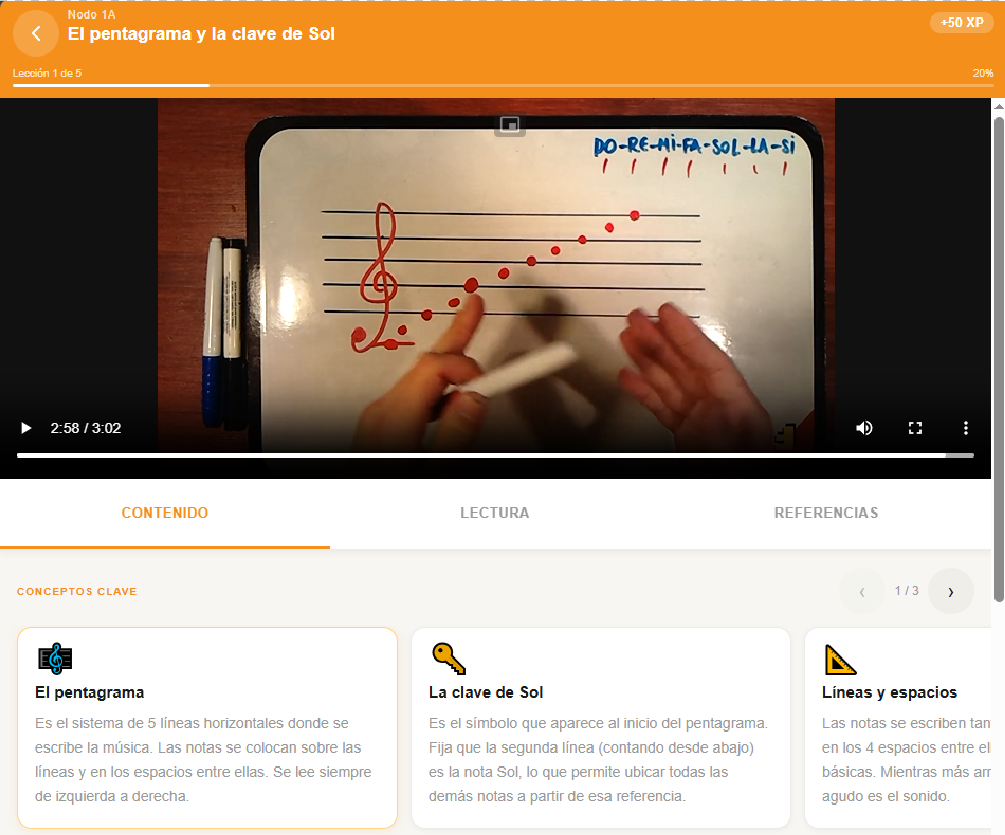
\includegraphics[width=0.45\textwidth]{Imagenes/MaterialAprendizajeFrontend.png}
    \caption{Módulo de lección teórica: Renderizado dinámico del material pedagógico a partir del objeto \texttt{JSONB} provisto por la RPC.}
    \label{fig:material_aprendizaje}
\end{figure}

\begin{figure}[htbp]
    \centering
    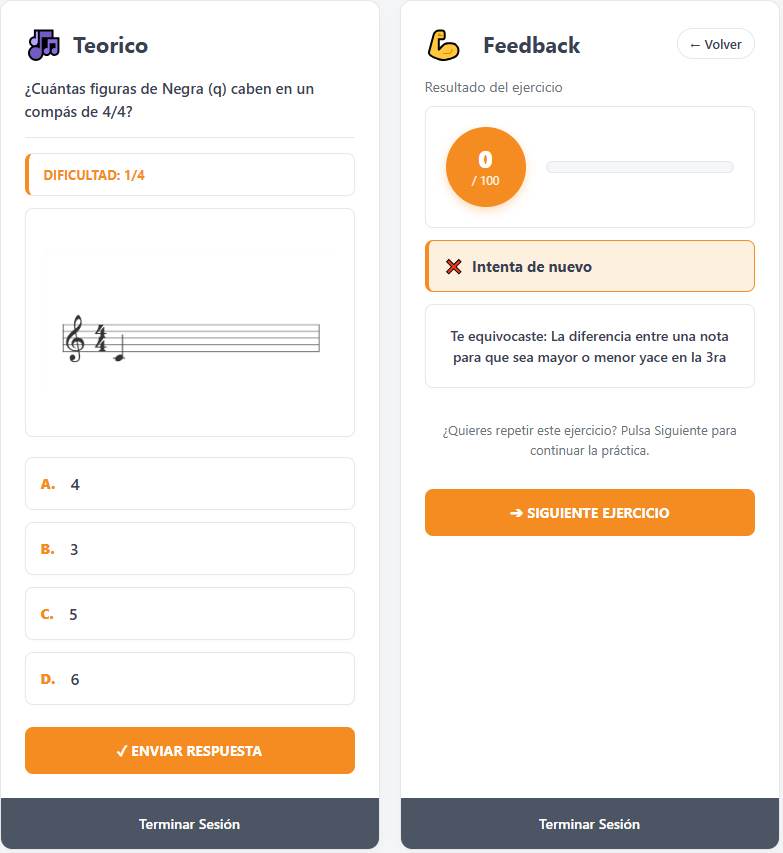
\includegraphics[width=0.45\textwidth]{Imagenes/frontend_ejercicio.png}
    \caption{Módulo de evaluación adaptativa: Flujo de interacción para la resolución de ejercicios y solicitud de inferencia al motor DRL.}
    \label{fig:ejercicios}
\end{figure}

\subsection{Grafo Dirigido Acíclico (DAG)}
El dominio de la teoría musical se formalizó mediante un Grafo Dirigido Acíclico (DAG) definido como $G = (V, E)$, donde $V$ representa 23 unidades de conocimiento (nodos) y $E$ corresponde a 29 aristas que modelan relaciones de dependencia pedagógica entre los conceptos. Estas dependencias representan prerrequisitos recomendados para facilitar una progresión lógica del aprendizaje, pero no constituyen restricciones estrictas, ya que un estudiante puede acceder a contenidos posteriores si demuestra un nivel de dominio suficiente en las evaluaciones adaptativas.

Aunque el DAG completo contempla 23 unidades de conocimiento distribuidas en cinco niveles de dificultad, para el desarrollo y validación del sistema adaptativo se seleccionó un subconjunto de cuatro nodos fundamentales de teoría musical. Estos corresponden a \textit{Notas y Ritmos}, \textit{Intervalos}, \textit{Escalas Mayores y Menores} y \textit{Acordes Tríadas}, los cuales constituyen una base progresiva para el aprendizaje y permiten representar las principales relaciones de dependencia pedagógica utilizadas por el sistema de recomendación. La Fig.~\ref{fig:dag} muestra la estructura del subgrafo utilizado, donde las aristas representan las relaciones de prerrequisito entre los contenidos seleccionados.

La disponibilidad de un nodo $v_i \in V$ se clasifica dinámicamente según la regla:

\begin{equation}
State(v_i) = \begin{cases} 
\text{locked}, & \exists u \in Pred(v_i) \mid Prog(u) \neq \text{done} \\
\text{done}, & Prog(v_i) = \text{done} \\
\text{active}, & Prog(v_i) = \text{in\_progress} \\
\text{available}, & \text{en otro caso}
\end{cases}
\end{equation}

\begin{figure}[htbp]
    \centering
    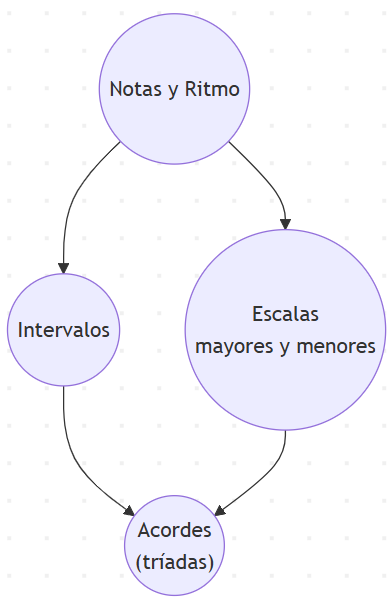
\includegraphics[width=0.25\textwidth]{Imagenes/grafo_dag.png}
    \caption{Subgrafo de dependencias pedagógicas utilizado para el entrenamiento y validación del sistema adaptativo.}
    \label{fig:dag}
\end{figure}

\subsection{Modelo Deep Learning}
El núcleo inteligente es un motor de recomendación basado en Deep Reinforcement Learning (DRL) que selecciona el ejercicio más apropiado para maximizar el aprendizaje en la zona de desarrollo proximal del estudiante.

\subsubsection{Detalle del modelo}

El modelo de aprendizaje por refuerzo interactúa de manera iterativa con el entorno de aprendizaje. En cada paso, recibe información sobre el progreso del estudiante, selecciona el siguiente ejercicio y observa el resultado obtenido. A partir de esta interacción, el agente ajusta su estrategia con el objetivo de recomendar secuencias de actividades que favorezcan el aprendizaje.

Para representar el progreso del estudiante, cada unidad de conocimiento se considera aprendida o no aprendida según un umbral predefinido. Las acciones del agente corresponden a la selección de uno de los ejercicios disponibles, mientras que la función de recompensa incentiva las recomendaciones que mejoran el dominio de los contenidos y penaliza aquellas que no producen avances significativos.

La función de recompensa se define como:
\begin{equation}
\begin{aligned}
R =\;&
1.0\,\mathbb{I}(\text{correcto})
+ 0.5\,\mathbb{I}(\text{mejoría}) \\
&+ 0.5\,\mathbb{I}\!\left(\left| d - d^{*} \right| \leq 1\right)
- 0.3\,\mathbb{I}\!\left(\left| d - d^{*} \right| > 2\right) \\
&+ 0.2\,\mathbb{I}(\text{poco practicado})
+ 0.1\,\mathbb{I}(\text{ejercicio nuevo})
\end{aligned}
\end{equation}
Se evaluaron DQN y PPO, seleccionándose \textbf{PPO} (\textit{Proximal Policy Optimization}) por su estabilidad, políticas estocásticas y convergencia balanceada entre exploración y explotación.

\subsubsection{Creación de dataset}
Ante la falta inicial de datos reales, se diseñó un proceso en dos etapas:
\begin{enumerate}
    \item \textbf{Encuestas:} Se aplicó un cuestionario anónimo mediante Google Forms, logrando recopilar 20 muestras correspondientes a estudiantes de enseñanza media pertenecientes a las comunas de Valdivia y Panguipulli. Los datos obtenidos permitieron estimar distribuciones de comportamiento, conocimientos previos y niveles iniciales de dominio musical. La recopilación no consideró información personal identificable, resguardando la privacidad de los participantes.
    \item \textbf{Simulación:} Se implementó un simulador probabilístico con perfiles ``desde cero'', ``parcial'' y ``avanzado'', encargado de generar trayectorias de aprendizaje sintéticas basadas en los patrones observados en la encuesta.
\end{enumerate}
Este enfoque generó un dataset sintético con aproximadamente 150,000 a 200,000 pasos de entrenamiento.

\subsubsection{Resultados del entrenamiento}
El entrenamiento se estructuró con una fase inicial de \textbf{Behavior Cloning}, donde una política inicial fue aprendida mediante la imitación de trayectorias expertas, siguiendo el enfoque de aprendizaje por imitación supervisado \cite{osa2018imitation}. En esta etapa, las demostraciones expertas fueron generadas mediante una política heurística basada en reglas pedagógicas del DAG, priorizando ejercicios disponibles, contenidos con bajo dominio y una progresión gradual de dificultad. El agente aprendió una aproximación inicial de esta estrategia antes de iniciar la optimización mediante Aprendizaje por Refuerzo Profundo.

Posteriormente, se realizó un entrenamiento iterativo con PPO durante 10,000 pasos de interacción con el entorno simulado. PPO demostró desarrollar políticas más estables frente a la incertidumbre educativa y un manejo adecuado de nuevos nodos, superando las tendencias conservadoras observadas previamente con el algoritmo DQN.


\subsection{Métricas de evaluación}

\subsubsection{Cómo se evaluará DRL}
La evaluación del agente DRL considerará métricas de progresión pedagógica y uso interactivo:
\begin{itemize}
    \item \textbf{Progreso de Aprendizaje (Proficiency):} Se medirá el incremento de la proficiencia estimando una meta de al menos un 15\% de mejora en el nivel de conocimientos.
    \item \textbf{Tasa de Continuidad:} Registro del uso ininterrumpido y la cantidad de sesiones a lo largo de las semanas de prueba.
    \item \textbf{Adaptabilidad de la Dificultad:} Análisis del ajuste dinámico entre la dificultad sugerida por el agente y el nivel real (\textit{performance}) del usuario.
\end{itemize}

\subsubsection{Cómo se evaluará la plataforma}
La evaluación general de SheetMusic incluirá percepciones directas de los usuarios (estudiantes y profesores):
\begin{itemize}
    \item \textbf{Usabilidad (Estudiantes):} Aplicación de la \textit{System Usability Scale} (SUS) para medir la accesibilidad e interfaz de usuario de la PWA.
    \item \textbf{Aceptación Tecnológica (Docentes):} Aplicación del instrumento TAM (\textit{Technology Acceptance Model}) para valorar la utilidad percibida y la facilidad de uso del panel de seguimiento pedagógico.
\end{itemize}